\chapter{Introduction} \label{chap:introduction}

The rising popularity of statically typed functional languages led to
the programming methodology of ``type-driven development'' (hereinafter referred to as TDD),
which is a style of development that revolves around the types of missing parts in
programs. The expressions users have not written yet, or ones they do not know
how to write, can be left as holes in their program, and the program still
compiles, with a warning that there are incomplete parts.
A hole is kind of expression, and since these languages are
statically typed, those holes have types. The parts
programmers have already written dictate what the types of the remaining parts should
be. These types can guide them when they try to fill the holes to complete the program.
In other words, TDD allows writing programs incrementally and top-down. This
not only lets them type-check programs at every step, but it also gives them clever
hints about the following steps, based on the types and the local
contexts.\footnote{Especially as dependent types gradually sneak into
mainstream languages, like they already have to Haskell~\cite{eisenberg} and
Scala~\cite{scalaDep}, we predict that TDD will only get more popular.}
This idea was originally born in the world of proof assistants, and then it was
borrowed by more practical functional languages.
Interactive editing based on this idea has been used in proof assistants for a long
time; the Edinburgh LCF system~\cite{lcf}, HOL and
Isabelle~\cite{isabelle} have allowed users to prove theorems
incrementally.\footnote{Propositions and types are distinct in these systems.}
Users type in commands called ``tactics'' that update the proof state by
changing the goal, or by creating subgoals.
Unlike the ones above, there are tactic-based proof assistants like
Coq~\cite{coq} that generate a Curry-Howard style proof term at the end; these
proof assistants have focused on changing the proof term indirectly.
Inspired by these systems, others arose which
provide a new interface and type theory that focuses on
changing the proof terms directly by incrementally building them
up.
% \footnote{Changing the proof term indirectly with tactics is also called
% backward reasoning, and incrementally building up the proof term is called
% forward reasoning.} % Dan doesn't agree with this.
One of the earliest such proof assistants was the ALF proof
editor~\cite{ALF}, and the idea was developed further in Epigram~\cite{epigram}
and Agda~\cite{agda}.
The ideas that are brewed in these proof assistants continue to inspire more
mainstream functional languages.

The traditional programming workflow either depended on saving a file and
trying to compile (or run) with every edit, or in the Lisp tradition it
depended on the read-eval-print loop (REPL). This has changed with the
advancement of integrated development environments (IDEs), programs that have
certain functionalities such as code completion, syntax checking, displaying
compiler error messages on their corresponding lines, searching in
documentation, etc.
Through these features, IDEs enable rapid feedback and interaction cycles
between the user and checking tools of the language and computation
environment, but they are different from TDD. While IDEs can also use types to
assist the user, they do not direct the entire development process around types
\emph{per se}.
TDD is not a program; it is merely a style of programming in which
the development process takes the form of a conversation between the
type-checker/compiler and the user's editor/IDE.  However, this requires
certain changes to the compiler, such as being able to type-check incomplete
expressions and definitions~\cite{tdd}.

The kind of change that is important for this work is the editor
interaction mode (or the IDE mode, as it is called in Idris~\cite{idris}) that
lets the editor talk to the compiler.\footnote{To avoid any confusion,
we should mention that there are two different parts of an editor interaction
mode. The first is a plugin to the editor, often written in the script language
of the editor, such as Emacs Lisp or VimL. The second part is a separate
program that does the heavy lifting of the editing features that work with the
language itself.  \texttt{ghc-mod} in Haskell and \texttt{agda-mode} in Agda would
be perfect examples for the second part. We can call these parts the frontend
and backend of the editor interaction mode, respectively.  When we talk about
the language the editor interaction mode is implemented, we mean the language
used in the backend, because the language used in the frontend depends on the
editor.}
There are various existing examples of compilers and editors that do this sort
of interaction:
Proof General~\cite{pg} and CoqIDE for Coq,
the Emacs mode~\cite{agdamode} for Agda,
the Emacs mode~\cite{idrismode} for Idris,
jEdit~\cite{isabellejedit} for Isabelle,
and the editor mode of Lean~\cite{lean}.\footnote{Haskell's typed holes in GHC
are exciting, their editor interaction features are not as polished as the ones
Agda and Idris have, since GHC/Haskell does not come with a built-in editor
interaction system.}
Idris has a special place among these proving languages since it tries to
prioritize general purpose programming. Compared to mainstream languages
that have mature IDEs, Idris still has an unusual standing since it also is a
proof assistant~\cite{idrisfaq}.
This unique position of Idris provides motivation for editor features on par
with mature IDEs for other languages, as well as the TDD-style development
workflow via editor actions.
Therefore, our work strives to bring the long-standing traditions of proof
assistants and IDEs closer together, by introducing the ``edit-time tactics''
feature.  The word ``edit-time'' is a wordplay on the terms ``compile time''
and ``run time'', and it means that we run the tactics when we are still
writing our program in the editor.
The area of bringing IDE features to proof assistants is not new~\cite{ctcoq,
developingReuse, realTheoremProvers, toolSupport}, but it has been focusing
on their usefulness as proof tools, not necessarily how they can help
mainstream programmers. In contrast, we take tactics from proof assistants
and see how they can help type-driven developers.

Before we proceed to describe our work,
it is imperative to understand what exactly an editor action is.
Editor actions are commands in the editor that make a meaningful
change in the our code, or ones that give us some information about our
code. For example, if we are trying to define a function to compute the height
of a binary tree, we can just start by writing the type for the function.

\vspace{1em}
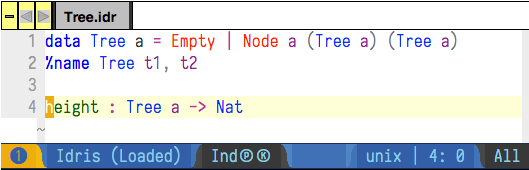
\includegraphics[scale=0.6]{edit1}

Note that initially we only declared the type of the function, and nothing
else. To get an initial incomplete definition, we can run the editor action
``Add initial match clause to type declaration,'' while the cursor is on the
type declaration.

\vspace{1em}
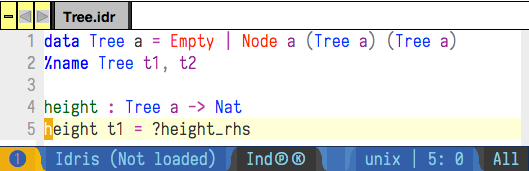
\includegraphics[scale=0.6]{edit2}

Now we have a definition for \fn{height} that takes one argument \bn{t1}, and
returns \hole{height\_rhs}. This is clearly incomplete; we want to change
the return value based on what \bn{t1} is. So the next step would be to inspect
what values \bn{t1} can take. We can place the cursor on \bn{t1} and then run
the editor action ``Case split pattern variable.''

\vspace{1em}
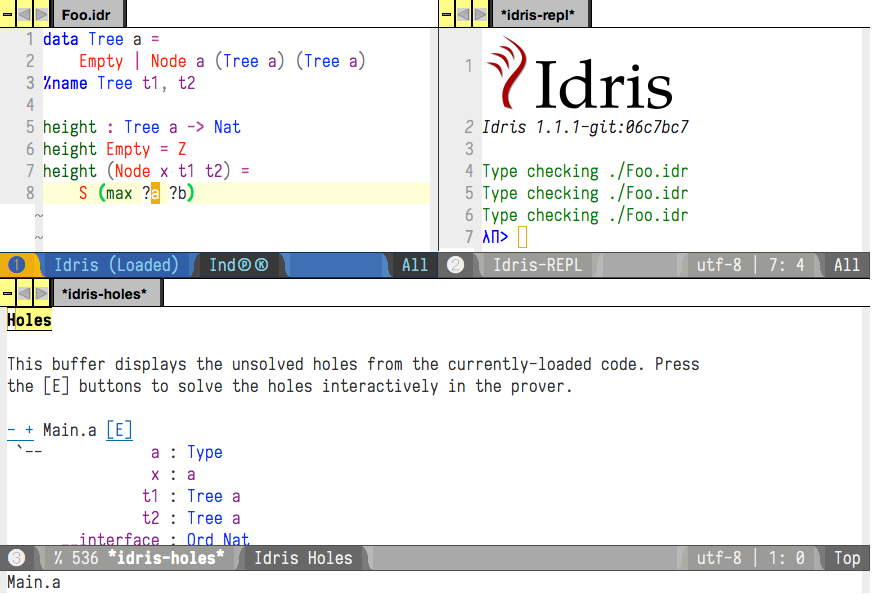
\includegraphics[scale=0.6]{edit3}

Now we have two holes that we have to complete, namely \hole{height\_rhs1} and
\hole{height\_rhs2}. When the cursor is on one of the holes, we can run the
editor action ``Display type'' and see what type of expression should replace
the hole, and what names are in the local context, i.e. are available to use
when writing that expression.

\vspace{1em}
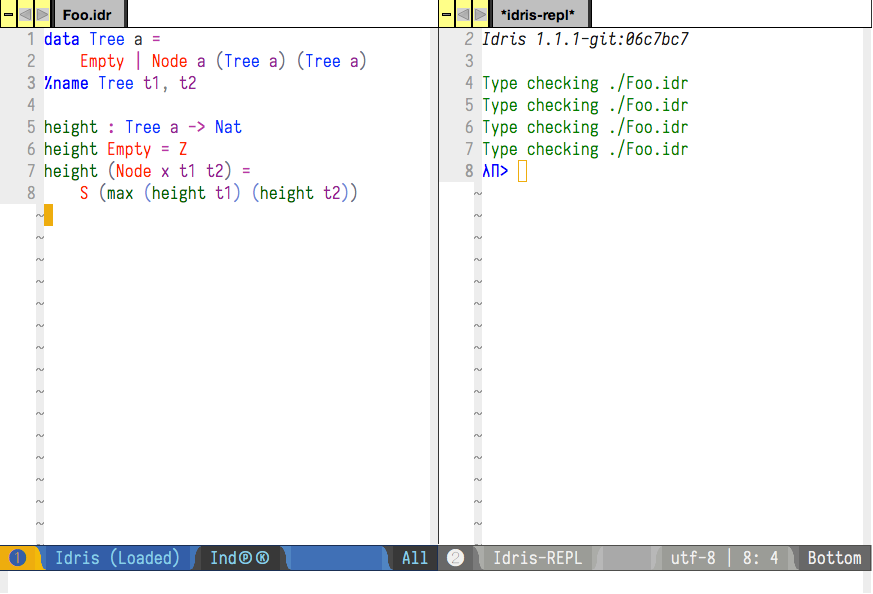
\includegraphics[scale=0.6]{edit4}

We complete the function by filling the holes by writing the expressions.

\vspace{1em}
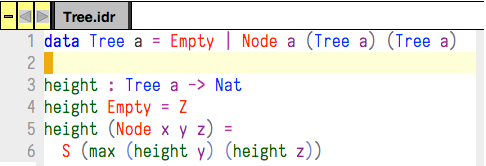
\includegraphics[scale=0.6]{edit5}

This example should show how much editor actions can shape our
programming experience.

\section{Motivation}

Now that we are familiar with what an editor action is, we can describe the problem
our project solves. The editor actions we reviewed above are features embedded
in the compiler. If you want to define a new action, the only way possible is
to change the compiler source code, build your own version of the compiler,
and then edit the source code of your editor mode to use that feature you
added. This is far from ideal: no one should have to fork a compiler
just to add a custom editor action. Maintaining a compiler fork and
navigating through the compiler source code are usually not in the skill sets
of most users.
Another drawback is that users would have to learn Haskell and recompile the
entire Idris system every time they want to define a custom editor action.

Therefore, we want to give users a way to write custom editor actions. Our
solution for this is to make use of elaborator reflection~\cite{elabref,leanmeta} in
Idris, which is a metaprogramming machinery that allows users to automate the
construction of proofs and programs, by reflecting the elaborator
monad~\cite{idris} in the Idris compiler. Christiansen and Brady showed that
this mechanism is powerful enough to replace the old tactic
language~\cite{elabref} that existed in the previous versions of Idris, which is
now deprecated in favor of elaborator reflection.

Elaborator reflection adds a primitive monad \Elab\ to Idris itself, in which
type-checking and normalizing terms, looking up types and definitions of
functions are monadic actions.\footnote{These monadic actions are still called
tactics, especially if they change the goal queue or the local context, hence the
title of this thesis. Note that whenever we use the word ``tactic'' in the
context of Idris, we exclusively refer to the monadic \Elab\ actions, not the
old tactic language.}
Our thesis argues that these actions provide a nice interface with which users
can define their custom editor actions. This has the following advantages:

\begin{itemize}
\item Implementations of the Idris editor actions mentioned above are
built in to the compiler, and they are written in Haskell. Our work will allow
us to rewrite them in Idris as \Elab\ actions. This way, we can remove these
parts from the compiler and move them into an Idris library.
\item The abilities of the editor interaction mode are extended from the
current built-in features to anything that can be done with tactics. This
allows library and DSL authors to provide domain-specific editor actions.
\item Defining editor actions with a monadic interface allows us to
compose them easily. For instance, if we had case-splitting as an
\Elab\ action, we could define a tactic to case-split on many arguments at the
same time.
\item More people can extend Idris; contributing to the Idris standard library
  or publishing a library of editor actions is much easier than extending the
    compiler itself.
\end{itemize}

To see what an edit-time tactic would look like, let's see an actual example in Emacs.

\vspace{1em}
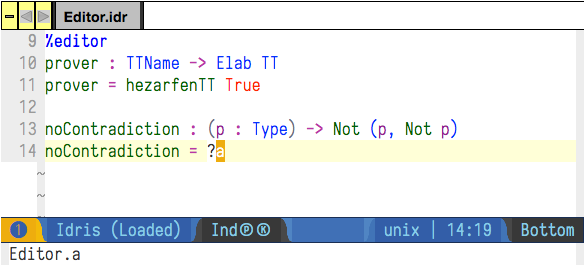
\includegraphics[scale=0.6]{hezarfen1}

In this example, we have defined an editor action \fn{prover} using the tactic
we explain in \autoref{sec:hezarfen}, set up an Emacs shortcut for it, and then
run it on a hole that we want to fill, using the tactic. We get the following
result:

\vspace{1em}
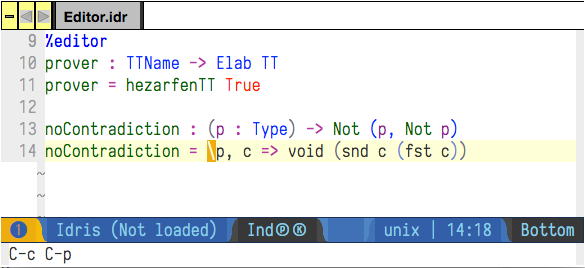
\includegraphics[scale=0.6]{hezarfen2}

\section{Contributions}

We make the following specific
contributions in this thesis:
\begin{itemize}
\item We extend the primitive \Elab\ monad with the necessary primitive monadic
actions that make writing an editor action with elaborator reflection possible
(\autoref{sec:stdlib}).
\item We define an Idris interface (or \emph{type class} in Haskell terminology)
called \ty{Editorable} for serializing and deserializing Idris expressions.
For the reflected type that represents the core language terms of Idris,
implementations of this interface are primitives (\autoref{sec:types}).
\item We extend the Idris compiler to track the association between source code
  and typing contexts (\autoref{sec:extendIState}).
\item The current proof search mechanism in Idris is not particularly advanced.
We write an alternative proof search tactic called Hezarfen, a full-blown
theorem prover for intuitionistic propositional logic, based on Dyckhoff's
LJT~\cite{ljt}, and then we show how to use this on holes when we are in
the editor (\autoref{sec:hezarfen}).
\item We define an add clause tactic that can be run from the editor, which can
replace the hard-coded add clause editor action (\autoref{sec:addClause}).
\end{itemize}

Some of the features we implemented in this thesis have already made their way to
the Idris compiler, and the rest also will once they are reviewed by the
other Idris contributors.

We envision three different audiences for this thesis:
\begin{enumerate}[(1)]
\item Idris programmers who use editor actions in their editor, who will now
  have access to more editor actions. For them, reading the applications of
edit-time tactics in \autoref{chap:applications} would be the most helpful.
\item Advanced Idris programmers who want to write simple editor actions, using
  the common Idris types and reflected types. More advanced Idris programmers
    may want to write more complex editor actions that involve data types
    that they define.
    They may want to read \autoref{chap:design} in order to understand the
    design of our feature and what should be taken into account when defining
    such data types.
\item Compiler developers and contributors for Idris and other
  dependently-typed languages.  They may want to read
    \autoref{chap:implementation} in order to observe what we needed to change
    in the compiler, and how they can add this feature to a different language.
\end{enumerate}

Now that we have gotten a taste of edit-time tactics and we know what to look
for while reading this thesis, we review the basics of the Idris
programming language and its metaprogramming machinery in
\autoref{chap:background}.
We discuss the design of the edit-time tactics feature in
\autoref{chap:design} and their implementation in
\autoref{chap:implementation}.

Before we move on the other chapters, it might be helpful to take a brief look
at the typographic conventions we use in this thesis: when we have code
excerpts, we will use a monospace font.  Keywords will be written in \kw{black
boldface}, types will be \ty{blue}, constant and function names will be
\fn{green}, data type constructors and primitives will be \dt{red}, bound
variables will be \bn{purple}, holes will be
\texttt{\IdrisMetavar{cyan}}, and comments will be
\cm{dark gray}.\footnote{We are following the color conventions in Conor McBride's
Epigram paper~\cite{epigram}.} We will have code excerpts in different
programming languages such as Idris, Haskell, and Emacs Lisp in this thesis.
For that reason we will always explicitly state what language the code is in,
but we will use the same highlighting for all of them.
